%!TEX root=../GaugeCNNTheory.tex


\subsection{The tangent bundle \textit{TM} and frame bundle \textit{FM}}
\label{sec:GL_associated_bundles}


Any differentiable (and thus any Riemannian) manifold $M$ is canonically equipped with its tangent bundle $\TM$ and the (general) frame bundle $\FM$, consisting of all local reference frames of the tangent spaces.
The two bundles are naturally associated to each other, with their structure group a-priori given by $\Aut(\R^d) = \GL{d}$.
This fact will be emphasized by ``reconstructing'' $\TM$ from $\FM$ via an associated bundle construction which will later allow us to define associated feature vector bundles.
To clearly separate the concepts introduced and assumptions made, we will describe $\TM$ and $\FM$ here as $\GL{d}$-bundles.
The following Section~\ref{sec:G_associated_bundles} will additionally assume a $G$-structure imposed on $\TM$ and $\FM$, which will establish them as $G$-bundles.
While bundles are locally trivializable by definition, we will take the specific trivializations for now as granted and postpone their exact definition to Section~\ref{sec:bundle_trivializations}.




\paragraph{Tangent bundle \textit{TM}:}

Any smooth manifold $M$ comes with a set of tangent spaces $\TpM\cong\R^d$.
Their disjoint union%
\footnote{%
    The disjoint union $\coprod_{p\in M} \TpM = \bigcup_{p\in M} \left\{(p,v) \,|\, v\in \TpM\right\}$ of tangent spaces can be thought of as ``remembering'' from which particular tangent space $\TpM$ a certain vector $v\in \TM$ originates, which is necessary for the definition of the projection map $\piTM$.
}
\begin{align}
    \TM\ :=\, \coprod_{p\in M} \TpM \,,
\end{align}
together with a canonically given smooth structure and projection map, defines a smooth fiber bundle known as the \emph{tangent bundle}.
The projection map ${\piTM: \TM\to M}$ is thereby given by the obvious choice ${\piTM(v)=p}$ for $v\in \TpM$.
As derived in Appendix~\ref{apx:coordinate_bases}, local trivializations $\PsiTM: \piTM^{-1}(U) \to U\times \R^d$ of the tangent bundle are canonically induced by charts $x:U\to V\subseteq \R^d$ of the manifold.
We can therefore take the trivializability of $\TM$ as granted and postpone their discussion to Section~\ref{sec:bundle_trivializations}.
A smooth structure on $\TM$ is induced from the smooth structure of $M$ via the above mentioned trivializations from charts.
We skip the technicalities on this construction and refer the interested reader to~\cite{schullerGeometricalAnatomy2016,nakahara2003geometry}.

The thus defined tangent bundle is a \emph{vector bundle} since its typical fiber $\R^d$ is a vector space.
Tangent vector fields, describing for instance a flow on $M$, are formalized as sections $\sigma: M\to \TM$ of the tangent bundle.
Smooth global sections of vector bundles always exist; a standard example is the zero section which assigns the zero vector of $\TpM$ to each $p\in M$.
We want to emphasize that the tangent spaces -- and therefore the tangent bundle -- are defined without reference to coordinate frames, such that sections describe vector fields in a coordinate free way.

After introducing the tangent frame bundle $\FM$ below, we will come back to the tangent bundle and its explicit construction as associated $\GL{d}$-bundle which emphasizes its coordinate free nature.
In Section~\ref{sec:G_associated_bundles} we will analogously construct $\TM$ as a associated $G$-bundle to a $G$-structure $\GM$.


\begin{figure}
    \centering
    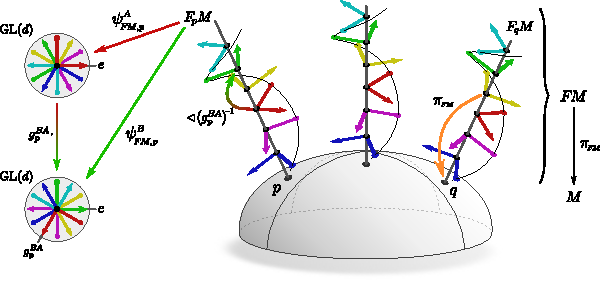
\includegraphics[width=1.\columnwidth]{figures/frame_bundle.pdf}
    \vspace*{-1ex}
    \caption{\small
        A graphical interpretation of the frame bundle $\FM$ over~$M$ and its trivializations.
        The fiber~$\FpM$ over~$p$ is defined as the space of all possible reference frames of~$\TpM$.
        All frames in $\FpM$ are by the projection map $\piFM$ being mapped to that point $p$ in $M$ to which the fiber is attached.
        The fibers $\FpM$ are isomorphic to $\GL{d}$, but come without an origin which would distinguish a preferred choice of reference frame.
        Gauges $\psiFMp^A: \FpM \to \GL{d}$ or $\psiFMp^B: \FpM \to \GL{d}$, introduced in Section~\ref{sec:bundle_trivializations} below, identify the fibers with $\GL{d}$, thereby specifying a preferred frame.
        Different gauges are related by gauge transformations $g_p^{BA} \in \GL{d}$.
        We need to warn the reader about two potential misconceptions:
        Firstly, the frames in different fibers are a-priori not identified with each other in a canonical way, which the redundant colors might suggest.
        Secondly, to minimize clutter, the visualization shows only right-handed, orthonormal frames instead of all possible reference frames.
        As we will discuss in the following Section~\ref{sec:G_associated_bundles}, the shown orthonormal, right-handed frames would correspond to a $G$-structure $\GM$ (a principal $G$-subbundle of $\FM$) for the structure group $G=\SO2$.
        }
    \label{fig:frame_bundle}
\end{figure}

\paragraph{Frame bundle \textit{FM}:}
The space of local reference frames of all tangent spaces $\TpM$ forms the (tangent) \emph{frame bundle}.
Consider the spaces of reference frames (ordered bases) of the individual tangent spaces $\TpM$:
\begin{align}
    \FpM\ :=\ \pig\{ \big[e_{1},\dots,e_{d}\big]\, \pig|\ \{e_{1},\dots,e_{d}\}\ \text{is a basis of } \TpM \pig\}
\end{align}
The frame bundle is defined as their disjoint union $\FM := \coprod_{p\in M} \FpM$ together with the projection map $\piFM: \FM\to M$ which sends frames in $\FpM$ to $p$ and a smooth structure induced from $\TM$.
The typical fiber of the frame bundle is
the general linear group $\GL{d}\cong \FpM$, i.e. the group of invertible $d\!\times\!d$ matrices whose linearly independent columns can be thought of as defining a frame of $\R^d$.
As the frame bundle is constructed from the tangent bundle, its local trivializations $\PsiFM: \piFM^{-1}(U) \to U \times \GL{d}$ are immediately induced from those of $\TM$; see Section~\ref{sec:bundle_trivializations}.
Fig.~\ref{fig:frame_bundle} shows a graphical interpretation of the frame bundle.


Smooth local sections $\sigma:U\to\piFM^{-1}(U)\subseteq \FM$ of the frame bundle map points $p\in U$ to frames in $\FpM$.
They define smooth local frame fields, that is, smoothly varying choices of reference frames for $\TpM,\ p\in U$; visualized in Fig.~\ref{fig:gauge_trafos_manifold}.
As argued in Eq.~\eqref{eq:framefield_gauge_equivalence}, a choice of frame field on $U$ is \emph{equivalent} to a choice of gauge or local trivialization on $U$.
This implies that global frame fields exist only if $\FM$ -- and thus $\TM$ -- are trivial.
We will discuss this equivalence in more depth in Section~\ref{sec:bundle_trivializations}.

A~transitive and free right action on the individual fibers $\FpM\cong\GL{d}$ of the frame bundle is naturally given by the change of frames defined in Eq.~\eqref{eq:frame_rightaction}~\cite{schullerGeometricalAnatomy2016}.
The corresponding action
\begin{align}\label{eq:rightaction_FM}
    \lhd:\ \FM\times \GL{d} \to \FM, \quad
    \big( [e_i]_{i=1}^d,\ g \big)
    \ \mapsto\ 
    [e_i]_{i=1}^d\! \lhd g \ :=\ 
    \left[ \sum\nolimits_j e_j\, g_{ji} \right]_{i=1}^d
\end{align}
on $\FM$ as a whole makes the frame bundle to a principal $\GL{d}$-bundle.
The lack of origin or preferred identity element of the fibers $\FpM$ as $\GL{d}$-torsors reflects the inherent ambiguity of reference frames.










\paragraph{\textit{TM} as GL(\textit{d})-associated vector bundle (\textit{FM}$\boldsymbol{\times \mathds{R}^d)/}$GL(\textit{d})\,:}
In Section~\ref{sec:gauges_gauge_trafos} we expressed~tangent vectors in $\TpM$ in terms of their coefficients in $\R^d$ relative to some reference frame.
The particular choice of frames was thereby irrelevant since the transformation of the coefficients in Eq.~\eqref{eq:components_leftaction} cancels with the transformation of reference frames in Eq.~\eqref{eq:frame_rightaction} such that $v = \sum_i v^A_i e^A_{i} = \sum_i v^B_i e^B_{i}$ are equivalent coordinate representations of the same coordinate free vector $v\in \TpM$.
Following this idea, one can construct the tangent bundle from the frame bundle by pairing reference frames with coefficient vectors and taking a quotient to collapse the resulting redundant descriptions of tangent vectors relative to different frames to one unique element.

In order to construct the tangent bundle in this way, consider the product $\FM\times\R^d$ which can be seen as a fiber bundle with base space $M$ and a typical fiber $\GL{d}\times\R^d$.
This bundle consists of pairs of (mutually unrelated) reference frames and coefficients.
Motivated by the equivalent expression of tangent vectors in different reference frames we define the \emph{equivalence relation}%
\footnote{\label{footnote:equiv_rel}%
    An \emph{equivalence relation} on a set $X$ is a binary relation $\sim$ which is
    \emph{reflexive} ($x\!\sim\! x$),
    \emph{symmetric} ($x\!\sim\! y \Leftrightarrow y\!\sim\! x$) and
    \emph{transitive} ($x\!\sim\! y \wedge y\!\sim\! z \Rightarrow x\!\sim\! z$).
    It defines a partitioning of $X$ into \emph{equivalence classes} $[x] := \{y\in X | x\sim y\}$ of elements $x\in X$.
    The space of equivalence classes $X/\!\!\sim\ := \{[x] \,|\, x\in X\}$ is called the \emph{quotient set} of $X$ by $\sim$.
}
\begin{align}\label{eq:equiv_relation_TM}
    \big([e_i]_{i=1}^d,\,\mathscr{v}\big)\ \sim_{\GL{d}}\, \big([e_i]_{i=1}^d\!\lhd g^{-1},\, g\cdot \mathscr{v}\big) \qquad\forall\, g\in \GL{d}
\end{align}
on $\FM\times\R^d$.
As an equivalence relation, it partitions $\FM\times\R^d$ into \emph{equivalence classes} $\big[[e_i]_{i=1}^d,\,\mathscr{v}\big]$.
The space of these equivalence classes is the quotient space $(\FM\times\R^d)/\GL{d}$.
The projection map
\begin{align}\label{eq:associated_TM_proj}
    \pi_{\scalebox{.75}{$\sim_{\GL{d}}$}}:\ 
    (\FM\times\R^d)/\GL{d} \to M,\ \ 
    \big[[e_i]_{i=1}^d,\,\mathscr{v}\big] \mapsto \piFM\!\left([e_i]_{i=1}^d\right) \,,
\end{align}
which is induced from the frame bundle, makes $(\FM\times\R^d)/\GL{d}$ to a fiber bundle with base space $M$ and typical fiber~$\R^d$.
Note that the projection map in Eq.~\eqref{eq:associated_TM_proj} is well defined as it is independent of the representative of the equivalence class, i.e.
$\pi_{\scalebox{.75}{$\sim_{\GL{d}}$}}\left(\big[[e_i]_{i=1}^d\lhd g^{-1},\, g\cdot \mathscr{v}\big]\right) := \piFM\left([e_i]_{i=1}^d\!\lhd g^{-1}\right) = \piFM\left([e_i]_{i=1}^d\right)$,
where we used that the right action $\lhd$ preserves the fibers of $\FM$.
The vector space structure of $\R^d$ makes $(\FM\times\R^d)/\GL{d}$ to a vector bundle with linear combinations within the same fiber being defined by
\begin{align}\label{eq:associated_bdl_linear_combination}
    \alpha \big[[e_i]_{i=1}^d,\,\mathscr{v}\big] + \beta \big[[e_i]_{i=1}^d,\,\mathscr{w}\big]
    \ :=\ \big[[e_i]_{i=1}^d,\,\alpha\mathscr{v} + \beta\mathscr{w} \big] \,,
\end{align}
for arbitrary $\alpha,\beta\in\R$ and $\mathscr{v},\mathscr{w}\in\R^d$.
This definition is easily checked to be independent of the choice of representative in both summands.

The thus defined bundle is isomorphic to the tangent bundle,
\begin{align}
    \TM\, \cong\, (\FM\times\R^d)/\GL{d} \,,
\end{align}
with the vector bundle $M$-isomorphism given by the fiber wise linear map
\begin{align}\label{eq:A_TM_isomorphism}
    \chi:(\FM\times\R^d)/\GL{d}\ \to \TM,\ \ \ \left[[e_i]_{i=1}^d,\, \mathscr{v}\right] \mapsto \sum_{i=1}^d \mathscr{v}_i e_i
\end{align}
which takes some representative tuple of frame and coefficient vector from the equivalence class and maps them to the corresponding tangent vector.
By the definition of the equivalence relation $\sim_{\GL{d}}$, this function is independent of the choice of representative, that is,
$
    \forall g\in \GL{d}: \ 
    \chi\left( \big([e_i]_{i=1}^d\lhd g^{-1},\, g\cdot \mathscr{v}\big) \right) = 
    {\sum_i (g\!\cdot\!\mathscr{v})_i \left([e_j]_{j=1}^d\!\lhd g^{-1}\right)_i} =
    \sum_i \mathscr{v}_i e_i \, ;\,
$
cf.~Eq.~\eqref{eq:vector_in_different_bases}.
As discussed in~\cite{schullerGeometricalAnatomy2016}, the inverse is given by taking a tangent vector, projecting it on an arbitrary frame and taking the equivalence class.


The bundle $(\FM \times \R^d) / \GL{d}$ is by construction associated to $\FM$ as $\GL{d}$-bundle, that is, it has the same transition functions in $\GL{d}$ as $\FM$, as we will derive in Section~\ref{sec:bundle_trivializations}.
The construction of $\TM$ as quotient $(\FM\times\R^d)/\GL{d}$ emphasizes the \emph{coordinate free} nature of the tangent bundle in a very intuitive way:
it considers all possible choices of coordinatizations of the tangent spaces and treats them as being equivalent by taking a quotient.
